% Options for packages loaded elsewhere
\PassOptionsToPackage{unicode}{hyperref}
\PassOptionsToPackage{hyphens}{url}
%
\documentclass[
]{article}
\usepackage{lmodern}
\usepackage{amssymb,amsmath}
\usepackage{ifxetex,ifluatex}
\ifnum 0\ifxetex 1\fi\ifluatex 1\fi=0 % if pdftex
  \usepackage[T1]{fontenc}
  \usepackage[utf8]{inputenc}
  \usepackage{textcomp} % provide euro and other symbols
\else % if luatex or xetex
  \usepackage{unicode-math}
  \defaultfontfeatures{Scale=MatchLowercase}
  \defaultfontfeatures[\rmfamily]{Ligatures=TeX,Scale=1}
\fi
% Use upquote if available, for straight quotes in verbatim environments
\IfFileExists{upquote.sty}{\usepackage{upquote}}{}
\IfFileExists{microtype.sty}{% use microtype if available
  \usepackage[]{microtype}
  \UseMicrotypeSet[protrusion]{basicmath} % disable protrusion for tt fonts
}{}
\makeatletter
\@ifundefined{KOMAClassName}{% if non-KOMA class
  \IfFileExists{parskip.sty}{%
    \usepackage{parskip}
  }{% else
    \setlength{\parindent}{0pt}
    \setlength{\parskip}{6pt plus 2pt minus 1pt}}
}{% if KOMA class
  \KOMAoptions{parskip=half}}
\makeatother
\usepackage{xcolor}
\IfFileExists{xurl.sty}{\usepackage{xurl}}{} % add URL line breaks if available
\IfFileExists{bookmark.sty}{\usepackage{bookmark}}{\usepackage{hyperref}}
\hypersetup{
  pdftitle={Metaheurísticas de trayectoria para la planificación de la recogida de residuos para reciclaje minimizando el impacto ambiental},
  pdfauthor={Pablo Hidalgo García},
  hidelinks,
  pdfcreator={LaTeX via pandoc}}
\urlstyle{same} % disable monospaced font for URLs
\usepackage[margin=1in]{geometry}
\usepackage{longtable,booktabs}
% Correct order of tables after \paragraph or \subparagraph
\usepackage{etoolbox}
\makeatletter
\patchcmd\longtable{\par}{\if@noskipsec\mbox{}\fi\par}{}{}
\makeatother
% Allow footnotes in longtable head/foot
\IfFileExists{footnotehyper.sty}{\usepackage{footnotehyper}}{\usepackage{footnote}}
\makesavenoteenv{longtable}
\usepackage{graphicx,grffile}
\makeatletter
\def\maxwidth{\ifdim\Gin@nat@width>\linewidth\linewidth\else\Gin@nat@width\fi}
\def\maxheight{\ifdim\Gin@nat@height>\textheight\textheight\else\Gin@nat@height\fi}
\makeatother
% Scale images if necessary, so that they will not overflow the page
% margins by default, and it is still possible to overwrite the defaults
% using explicit options in \includegraphics[width, height, ...]{}
\setkeys{Gin}{width=\maxwidth,height=\maxheight,keepaspectratio}
% Set default figure placement to htbp
\makeatletter
\def\fps@figure{htbp}
\makeatother
\setlength{\emergencystretch}{3em} % prevent overfull lines
\providecommand{\tightlist}{%
  \setlength{\itemsep}{0pt}\setlength{\parskip}{0pt}}
\setcounter{secnumdepth}{5}

\title{Metaheurísticas de trayectoria para la planificación de la recogida de
residuos para reciclaje minimizando el impacto ambiental}
\author{Pablo Hidalgo García}
\date{}

\begin{document}
\maketitle

\hypertarget{introducciuxf3n}{%
\section{Introducción}\label{introducciuxf3n}}

En la compleja sociedad moderna aparecen retos que es necesario abordar
y solucionar de la mejor forma posible para que la vida sea fácil y
llevadera. Además, existe una conciencia creciente acerca del impacto
medioambiental de nuestras actividades por lo que las soluciones a estos
retos deben tenerlo en consideración. Uno de esos muchos retos es la
gestión de los residuos. La sociedad de consumo moderna implica una alta
generación de residuos que es necesario procesar para reducir la huella
medioambiental así como evitar la aparición de enfermedades o las
incomodidades propias de la convivencia con los residuos. En el año 2017
se recogieron en España más de 22.000 toneladas de residuos (alrededor
de 460 kilogramos por habitante) y que da cuenta de la magnitud y la
dificultad en la gestión.

En áreas rurales o insulares en las que las diseminación de la
generación de residuos es más acusada, esta gestión es complicada en el
sentido de que los trayectos pueden ser amplios, la frecuencia de
recogida no puede ser diaria y debe adaptarse lo mejor posible al
comportamiento de la generación de los residuos. Por ello es fundamental
que la recogida de estos residuos se haga de la forma más eficiente
posible.

Se pueden distinguir dos formas en la que la recogida de los residuos se
puede mejorar. La primera de ellas es realizar inversiones que consigan
adaptar los recursos e infraestructuras disponibles (camiones de
recogida, puntos de recogida, plantas de procesamiento, etcétera) a los
patrones de generación de residuos; la segunda es optimizar la recogida
contando con los recursos ya existentes.

Es en este segundo enfoque en el que se incide en este trabajo, en
particular en optimizar las rutas que recorren los vehículos de recogida
de resiguos con el objetivo de recolectar la máxima cantidad de residuo
conforme a las restricciones de recursos ya existentes. Algunas de las
restricciones más habituales y determinantes pueden ser:

\begin{itemize}
\tightlist
\item
  plantas de procesamiento,
\item
  puntos de recogida (situación, distancia entre ellos, patrones de
  llenado),
\item
  vehículos de recogida (número, capacidad, etcétera),
\item
  horas de trabajo (habitualmente nocturnas).
\end{itemize}

De estas restricciones la más fuerte es el número máximo de horas de
trabajo que se consideran de 6.5 horas dejando un margen para cualquier
eventualidad. Esta restricción es obvia para que los trabajadores
descansen adecuadamente y, además, por la naturaleza de la recogida de
residuos, se fomenta la recogida durante los periodos nocturnos para
minimizar el impacto que estas actividades tienen sobre la población.

Este trabajo se desarrolla en este contexto tomando como escenario de
estudio la Isla de la Palma (Islas Canarias, España) aunque su
aplicación se puede extender y adaptar a cualquier otra área geográfica.
La información disponible son: patrones de generación de residuos,
emplazamiento de los contenedores y sus características, detalles de las
rutas, tiempo y coste y las restricciones de los recursos disponibles.
Existen tres puntos de origen y destino de las rutas situadas en tres
municipios de la Palma: Breña Alta, Mazo y Los Llanos. Cada vehículo
debe llevar a cabo una ruta diaria y, cada ruta se define como un
secuencia de puntos de recogida que deben ser visitados por cada
vehículo. Se considera que cada vez que un camión visita un punto de
recogida, éste recoge todo el residuo acumulado. Un supuesto general que
se ha aplicado es el de que no todos los puntos de recogida deben ser
visitados diariamiente. En zonas urbanas donde la generación de residuos
puede ser muy alta, probablemente se requerirá una visita diaria a todos
los puntos de recogida por lo que, en cualquier caso, los recursos
existentes (número de vehículos, por ejemplo) ha de estar acorde a
alcanzar este objetivo. Sin embargo, en zonas rurales o, como se trata
en este trabajo, insulares, no es necesario que la periodicidad de las
visitas sean diaras. Este escenario de estudio toma como punto de
partida el trabajo iniciado en (Expósito-Márquez et al. 2019).

Las principales contribuciones de este trabajo son:

\begin{enumerate}
\def\labelenumi{\arabic{enumi}.}
\tightlist
\item
  Propuesta de un algoritmo metaheurístico híbrido entre una búsqudda
  tabú y una búsqueda por vecindarios variables.
\item
  Comparativa del algoritmo propuesto con la ruta real y con
  (Expósito-Márquez et al. 2019)
\item
  Estudio del algoritmo bajo distintos escenarios.
\end{enumerate}

Este trabajo está organizado de la siguiente forma. La sección 2 hace un
revisión bibliográfica del problema. En la sección 3 se describen las
características del problema para definirlo de manera formal en la
sección 4. En la sección 5 se describe la solución propuesta para la
resolución del problema y, en la sección 6, se estudian los resultados
computacionales aplicados sobre el escenario de la Isla de la Palma.
Finalmente, en la sección 7 se dan las principales conclusiones y
trabajo futuro.

\hypertarget{revisiuxf3n-bibliogruxe1fica}{%
\section{Revisión bibliográfica}\label{revisiuxf3n-bibliogruxe1fica}}

El problema de la recogida de residuos, tal y como se discute en este
trabajo, se trata de encontrar la ruta óptima (es decir, qué puntos de
recogida debe visitar) para cada vehículo de recogida de forma que se
recoja la mayor cantidad de residuo. Este problema se puede englobar
dentro de los problemas conocidos como problema de enrutamiento de
vehículos (Vehicle Routing Problem o VRT) enunciado por primera vez en
(Dantzig and Ramser 1959) y que puede considerarse como una
generalización del problema del viajante (Traveling-Salesman Problem o
TSP) (Flood 1956).

En el problema del viajante (TSP en lo que sigue) se busca en su
formulación original, dada una lista de ciudades y las distancias entre
ellas, cuál es la ruta óptima (orden en el que deben ser visitadas)
pasando exactamente una vez por cada una de ellas. Aunque su formulación
sea como una optimización de rutas, sus aplicaciones van más allá de
este escenario en áreas como Este problema es útil por su aplicación
práctica en áreas como la planificación, la logística, la fabricación de
microchips o, con algunas modificaciones incluso en la secuenciación del
ADN (Punnen 2007).

El problema de enrutamiento de vehículos (VRP en lo que sigue) trata de
encontrar la mejor ruta para una flota de vehículos (y no solo uno, como
en el TSP) para satisfacer la demanda de un conjunto de clientes
conforme a un criterio de optimización. Este problema presenta algunas
variaciones (Golden, Raghavan, and Wasil 2008) como, por ejemplo,

\begin{enumerate}
\def\labelenumi{(\roman{enumi})}
\tightlist
\item
  Capacitated VRP: está disponible una flota homogénea de vehículos
  donde la restricción es la capacidad de cada vehículo,
\item
  VRP con ventana de tiempos: los clientes tienen que ser servidos en un
  intervalo de tiempo específico.
\end{enumerate}

En los problemas VRP tradicionales, el objetivo se trata desde un punto
de vista del impacto económico (habitualmente, se define algún tipo de
coste). Sin embargo, han surgido una familia de problemas denominados
\emph{Green Vehicle Routing Problems} (GVRP) caracterizados por tener en
cuenta la armonización entre el impacto económico y medioambiental.
Dentro de esta familia de problemas, se pueden ver tres grandes
categorías (Lin et al. 2014):

\begin{itemize}
\tightlist
\item
  G-VRP (Green-VRP): el objetivo es optimizar el consumo de la energía
  necesaria para el transporte,
\item
  Pollution Routing Problem (PRP): el objetivo es encontrar la mejor
  planificación de rutas desde el punto de vista de la contaminación, en
  particular, reduciendo las emisiones de carbono.
\item
  VRP en Reverse Logistics (VRPRL): estos problemas están relacionados
  con aspectos de la logística inversa (traslado de materiales apra su
  reciclado, reutilización o destrucción).
\end{itemize}

Este tipo de problemas entran dentro de la categoría de optimización
combinatoria y, debido a su complejidad, la obtención de soluciones
óptimas resulta complicado (o directamente inviable) cuando el tamaño
del problema es suficientemente grande. Por ello, las soluciones más
habituales en la bibliografía se desarrollan como algoritmos
metaheurísticos (Golden, Raghavan, and Wasil 2008). Los algoritmos
metaheurísticos son métodos capaces de desarrollar soluciones
aproximadas integrando procedimientos de búsqueda local y estructuras de
alto nivel para crear procesos capaces de escapar de soluciones locales
y realizar búsquedas robustas en el espacio solución (Gendreau and
Potvin 2010). Estos algoritmos se pueden clasificar en distintas
categorías (Birattari et al. 2001):

\begin{itemize}
\tightlist
\item
  métodos de trayectoria vs.~métodos discontinuos,
\item
  búsqueda basada en poblaciones vs.~búsqueda basada en un único punto,
\item
  métodos con memoria vs.~métodos sin memoria,
\item
  una vs.~varias estructuras de vecindarios,
\item
  función objetivo dinámica vs.~estática,
\item
  Inspirados en la naturaleza vs.~no inspirados en la naturaleza.
\end{itemize}

Algunos de estos algoritmos son la búsqueda tabú, el recocido simulado,
búsqueda en vecindarios variables o GRASP.

Algunas críticas habituales sobre estos algoritmos son, en algunos casos
de la su falta de elaboración conceptual, un diseño de experimentos
pobre e ignorancia de la literatura previa (Sörensen 2015).

Este trabajo toma como punto de partida el ya iniciado en
(Expósito-Márquez et al. 2019) acerca de la formulación matemática del
problema de la recogida de residuos y donde se desarrolla una solución
mediante el algoritmo metaheurístico Greedy Randomized Adaptative Search
Procedure (GRASP). También se estudia su comportamiento en la recogida
de residuos de papel y cartón (residuo azul) y plástico (resiudo
amarilla) en la isla de La Palma (Islas Canarias, España).

\hypertarget{descripciuxf3n-del-problema}{%
\section{Descripción del problema}\label{descripciuxf3n-del-problema}}

El problema de optimización consiste en el diseño de rutas que una flota
de vehículos debe seguir diariamente dentro de un horizonte de
planificación de varios días.

El problema se puede describir formalmente como un grafo completo
dirigido \(\mathcal{G} = (\Theta, A)\) donde
\(\Theta=\{\theta_1,\ldots, \theta_n\}\) se corresponde con el conjunto
de los \(n\) emplazamientos y
\(A=\{(\theta_i,\theta_j):\theta_i,\theta_j\in\Theta, i\neq j\}\), las
aristas del grafo de las que se conoce el tiempo de viaje \(d_{ij}>0\)
para cada arista \((\theta_i, \theta_j)\). Nótese que no tiene por qué
cumplirse la simetría entre tiempos de viaje, es decir que, en general,
no tiene porqué darse \(d_{ij} = d_{ji}\) para \(i\neq j\). Además, para
el conjunto \(\Theta\) se considera que \(\Theta = P \cup E\) de forma
que \(P\cap E = \emptyset\) donde \(P=\{P_1,P_2,\ldots,P_m\}\)
representa el conjunto de los \(m\) puntos de recogida y
\(E=\{e_1,e_2,\ldots,e_r\}\) el conjunto de los puntos de inicio o
destino de las rutas.

Se dispone de una flota de \(k\) vehículos expresados en el conjunto
\(\mathcal{V} = \{v_1,\ldots, v_k\}\). El origen y el destino de las
rutas que cada vehículo \(v\in\mathcal{V}\) puede realizar se denomina
como \(o(v)\in E\) y \(t(v)\in E\), respectivamente.

Se define el conjunto de días horizonte para los que se debe realizar la
planificación como \(\mathcal{H}=\{1,2,\ldots, h\}\).

Cada punto de recogida \(p \in P\) tiene asociada una función \(f_p(d)\)
normalizada del nivel de residuo que contiene. Aunque esta función puede
tomar cualquier expresión, en este trabajo se considera que esta función
tiene como ecuación

\[
f_p(d)=\min\{1, b_p + q_p \cdot d \}
\]

siendo \(b_p\in [0,1]\) el nivel de llenado del punto de recogida en el
día último día de recogida previo al día \(d\) y \(q_d\in [0,1]\) la
tasa de llenado del punto de recogida. Nótese que cuando la expresión
\(b_p + q_p \cdot d > 1\) significa que el punto de recogida está
desbordado (hay más residuo del que puede almacenar) de ahí la
utilización del mínimo en la función anterior.

En la siguiente sección se define en detalle la formulación matemática
del problema.

\hypertarget{formulaciuxf3n-matemuxe1tica}{%
\section{Formulación matemática}\label{formulaciuxf3n-matemuxe1tica}}

El problema se puede formular como un problema de programación entera
mixta (Mixed-Integer Programming o MIP). Necesitamos las siguientes
variables:

\begin{itemize}
\tightlist
\item
  \(X_{ijh}^v\): variable que toma valor \(1\) si el vehículo
  \(v\in\mathcal{V}\) va desde el punto \(\theta_i\) hasta el
  \(theta_j\) en el día \(h\in \mathcal{H}\) y 0 en caso contrario,
  \(\forall (\theta_i,\theta_j) \in A\)
\item
  \(Y_{ih}^v\): toma valor \(1\) si se visita el punto
  \(\theta_i\in\Theta\) por el vehículo \(v\in\mathcal{V}\) en el día
  \(h\in\mathcal{H}\) y 0 en caso contrario.
\item
  \(\mathcal{T}_{ih}\in\mathbb{R}\): tiempo de recogida del punto
  \(\theta_i\in\Theta\). Nótese que esta variable no depende de ningún
  vehículo ya que se considera que un punto de recogida solo se puede
  visitar por un único vehículo en un mismo día.
\end{itemize}

Así, las restricciones del problema son las siguientes:

\[
\sum_{j \in P} X_{o(v)jh}^v= 1, \quad v \in \mathcal{V}, h\in\mathcal{H}
\]

\[
\sum_{i \in P} X_{it(v)h}^v= 1 , \quad v \in \mathcal{V}, h\in\mathcal{H}
\]

\[
\sum_{j\in\Theta}X_{jkh}^v = \sum_{j\in\Theta}X_{kjh}^v, \quad v \in \mathcal{V}, h\in\mathcal{H}
\]

\[
\sum_{j\in\Theta} X_{ijh}^v = Y_{ih}^v , \quad i\in P, v \in \mathcal{V}, h\in\mathcal{H}
\]

\[
\sum_{v\in \mathcal{V}} Y_{ih}^v \leq 1, \quad i\in P,  h\in\mathcal{H}
\]

\[
T_{jh} \geq T_{ih} + s_i + t_{ij} - M\cdot \big(1-\sum_{v\in \mathcal{V}} X_{ijh}^v\big), \quad i,j \in \Theta, h\in\mathcal{H}
\]

\[
T_{ih} + s_i + t_{it(v)} \leq W_{vh}, \quad i\in \Theta, v \in \mathcal{V}, h\in\mathcal{H}
\]

\[
X_{ijh}^v \in \{0, 1\}, \quad i,j \in \Theta, v \in \mathcal{V}, h\in\mathcal{H}
\]

\[
Y_{ih}^v \in \{0, 1\}, \quad i\in P, v \in \mathcal{V}, h\in\mathcal{H}
\]

\[
T_{ih} \geq 0 ,\quad i\in\Theta, h\in \mathcal{H}
\]

El objetivo es

\[
\max \sum_{v \in V}\sum_{i\in P} \sum_{h\in H} F_i(\eta_{ih})\cdot Y_{ih}^v
\]

\hypertarget{soluciuxf3n-propuesta}{%
\section{Solución propuesta}\label{soluciuxf3n-propuesta}}

En esta sección se describe la solución propuesta. La formulación
matemática anterior mediante algoritmos exactos es intratable
computacionalmente cuando la dimensionalidad de los escenarios es alta
tal y como se muestra en (Expósito-Márquez et al. 2019) en un escenario
real.

La solución propuesta busca diseñar las rutas que deben seguir cada
vehículo cada uno de los días contenidos en el horizonte temporal. Para
ello se aplica en la marco general de la búsqueda en vecindarios
variables o VNS (Mladenović and Hansen 1997). VNS es un algoritmo
metaheurístico para resolver problemas de optimización combinatorios y
globales cuya principal idea es el cambio sistemático del vecindario de
búsqueda tanto en un fase de búsqueda local como en una fase de
perturbación que permita escapar de óptimos locales. Este algoritmo se
construye teniendo en cuenta tres hechos fundamentalesl algoritmo VNS
está basado en tres hechos fundamentales (Hansen et al. 2010): (1) un
mínimo local con respecto a una estructura de vecindario no lo es
necesariamente respecto de otra, (2) un mínimo global es un mínimo local
con respecto a todas las estructuras de vecindario posibles y (3) para
muchos problemas, el mínimo local con respecto a uno o varios
vecindarios están relativamente cercanos unos de otros.

Aunque hay diferentes variantes del algoritmo VNS, una de las
aproximaciones que más éxito han tenido es es la denominada General VNS
(Hansen et al. 2010). Su funcionamiento es el siguiente:

\textbf{Inicialización.} Seleccionar el conjunto de las estructuras de
vecindarios \(\mathcal{N}_k\) para \(k=1,\ldots, k_{max}\) que se usará
en la búsqueda; encontrar una solución inicial \(x\) y su valor de la
función objetivo \(f(x)\); asignar
\(x_{opt}\leftarrow x, f_{opt}\leftarrow f(x)\); elegir un critero de
parada.

\textbf{Repetir} lo siguiente hasta que se satisfaga el criterio de
parada:

\begin{enumerate}
\def\labelenumi{(\arabic{enumi})}
\tightlist
\item
  Asignar \(k\leftarrow 1\);
\item
  Repetir hasta que \(k=k_{max}\):

  \begin{enumerate}
  \def\labelenumii{(\alph{enumii})}
  \tightlist
  \item
    \textbf{Agitación}. Generar un punto \(x'\) aleatoriamente para el
    vecindario \(\mathcal{N}_k(x)\);
  \item
    \(l\leftarrow 1\);
  \item
    Repetir hasta que \(l=l_{max}\):

    \begin{enumerate}
    \def\labelenumiii{(\roman{enumiii})}
    \tightlist
    \item
      \textbf{Búsqueda local.} Encontrar el mejor vecino en
      \(\mathcal{N}_l(x')\) y denotarlo como \(x''\);
    \item
      \textbf{Cambio de vecindario.} Si \(f(x'') > f_{opt}\) hacer
      \(f_{opt}\leftarrow f(x'')\), \(x_{opt}\leftarrow x''\) y
      \(l\leftarrow l_{max}\); en otro caso \(l\leftarrow l + 1\);
    \end{enumerate}
  \item
    \textbf{Mover o no.} Si \(f(x'') < f_{opt}\), asignar
    \(k \leftarrow k + 1\); en caso contrario, \(k\leftarrow 1\).
  \end{enumerate}
\end{enumerate}

Este algoritmo GVNS tiene varias extensiones, entre ellas la hibridación
con otros algoritmos. Uno de los algoritmos metaheurísticos más
conocidos es la búsqueda tabú (Glover 1989). Esta algoritmo mantiene una
\emph{memoria} acerca de la búsqueda ya realizada para prohibir (tabú)
algunas soluciones recientes. Aunque se puede hibridar con GVNS de
distintas formas, en este trabajo utilizaremos una hibridación de forma
que el conjunto de soluciones vecinas esté limitado por la lista tabú.
Así, el algoritmo anterior quedaría como

\textbf{Inicialización.} Seleccionar el conjunto de las estructuras de
vecindarios \(\mathcal{N}_k\) para \(k=1,\ldots, k_{max}\) que se usará
en la búsqueda; encontrar una solución inicial \(x\) y su valor de la
función objetivo \(f(x)\); asignar
\(x_{opt}\leftarrow x, f_{opt}\leftarrow f(x)\); elegir un critero de
parada; definir un conjunto de soluciones tabú \(\mathcal{T}\).

\textbf{Repetir} lo siguiente hasta que se satisfaga el criterio de
parada:

\begin{enumerate}
\def\labelenumi{(\arabic{enumi})}
\tightlist
\item
  Asignar \(k\leftarrow 1\);
\item
  Repetir hasta que \(k=k_{max}\):

  \begin{enumerate}
  \def\labelenumii{(\alph{enumii})}
  \tightlist
  \item
    \textbf{Agitación}. Generar un punto \(x'\) aleatoriamente para el
    vecindario \(\mathcal{N}_k(x, \mathcal{T})\);
  \item
    \(l\leftarrow 1\);
  \item
    Repetir hasta que \(l=l_{max}\):

    \begin{enumerate}
    \def\labelenumiii{(\roman{enumiii})}
    \tightlist
    \item
      \textbf{Búsqueda local.} Encontrar el mejor vecino en
      \(\mathcal{N}_l(x')\) y denotarlo como \(x''\);
    \item
      \textbf{Cambio de vecindario.} Si \(f(x'') > f_{opt}\) hacer
      \(f_{opt}\leftarrow f(x'')\), \(x_{opt}\leftarrow x''\),
      \(l\leftarrow l_{max}\) y actualizar el conjunto tabú
      \(\mathcal{T}\); en otro caso \(l\leftarrow l + 1\);
    \end{enumerate}
  \item
    \textbf{Mover o no.} Si \(f(x'') < f_{opt}\), asignar
    \(k \leftarrow k + 1\); en caso contrario, \(k\leftarrow 1\).
  \end{enumerate}
\end{enumerate}

Para la aplicación del problema de optimización de recogida de residuos
enunciado es necesario definir la estructura de los vecindarios y cómo
se va a ir modificando la lista tabú.

Se consideran tres estructuras de vecindarios.

\begin{itemize}
\item
  Vecindario \(\mathcal{N}_1\): dada una ruta, se añade un nuevo punto
  de recogida teniendo en cuenta que un punto de recogida no debe
  aparecer en dos rutas del mismo día.
\item
  Vecindario \(\mathcal{N}_2\): se intercambian dos puntos de recogida
  entre dos días distintos.
\item
  Vecindario \(\mathcal{N}_3\): se intercambia un punto de recogida que
  aparece en una de las rutas por uno que no haya sido recogido teniendo
  en cuenta, de nuevo, que un punto de recogida no puede ser recogido
  dos veces en el mismo día.
\end{itemize}

Cabe señalar que una de las principales restricciones del problema es el
máximo tiempo que puede durar una ruta. Por tanto, en la búsqueda local
en el vecindario de una solución, en el caso de que se encuentre algún
vecino que, aunque tenga un valor de la función objetivo igual que la
mejor solución, si ésta supone una disminución en el tiempo total de las
rutas, se seleccionará esta solución.

Cada vez que se añade un punto de recogida a la solución, éste se
introduce en la lista tabú \(\mathcal{T}\). Además, es necesario definir
un parámetro \(\rho\) que especifique durante cuántas iteraciones un
punto de recogida no se considerará desde que fue introducido en la
lista \(\mathcal{T}\).

En realidad, el problema se puede dividir en dos partes: (1) asignar un
punto de recogida a una ruta y (2) elegir el orden adecuado en el que se
deben visitar los puntos de recogida en esa ruta. Para esta segunda
parte, se realiza una estrategia de mejora de la ruta mediante el
heurístico Lin-Kernighan (Helsgaun 2000) el cual se considera uno de las
mejores heurísticas para aplicar al problema TSP. Este heurístico se
implementa dentro de las soluciones obtenidas en las distintas
estructuras de vecindario.

\hypertarget{resultados-computacionales}{%
\section{Resultados computacionales}\label{resultados-computacionales}}

En esta sección se describen los resultados computacionales obtenidos en
el escenario de análisis. Los objetivos de este análisis son:

\begin{enumerate}
\def\labelenumi{\arabic{enumi}.}
\tightlist
\item
  Evaluar el comportamiento de la solución propuesta.
\item
  Comparar los resultados de la solución propuesta con la situación real
  actual y la solución propuesta en (Expósito-Márquez et al. 2019).
\item
  Evaluar el comportamiento de la solución bajo diversos escenarios.
\end{enumerate}

Los resultados computacionales que aparecen en esta sección se han
realizado en un ordenador equipado con un procesador Intel Core i7-8700
3.20GHz y 16 GB de memoria RAM. La implementación de la solución se ha
realizado utilizando el lenguaje de programación Python 3.8 y está
recogida en el repositorio \url{https://github.com/papabloblo/tfm}. Se
ha considerado un tiempo de ejecución de 4 horas, un tiempo asumible
para el que la empresa de recogida pueda obtener la planificación de las
rutas y llevarlas a cabo. Nótese que el horizonte temporal es de 5 días
así que, podría considerarse por parte de la empresa ejecutar el
algoritmo diariamiente para ir recalculando las rutas si eso fuese
posible y necesario utilizando como solución de inicial rutas
anteriores.

\hypertarget{resumen-de-los-datos}{%
\subsection{Resumen de los datos}\label{resumen-de-los-datos}}

El escenario sobre el que se aplica la solución propuesta es la Isla de
La Palma (Islas Canarias, España). Esta isla tiene una extensión de
708.32 \(km^2\) con una población de \(82.671\) habitantes {[}fuente:
\url{https://www.ine.es/jaxiT3/Datos.htm?t=2910\#!tabs-tabla}{]}. La
isla tiene como punto más elevado el Roque de los Muchachos (2426
metros). Está compuesta por 14 municipios. Su particular orografía y las
conexiones entre los municipios, hace que las distancias y tiempos de
viaje no sean simétricos. Además, se trata de una isla con un fuerte
componente turístico son una media de 140,000 turistas anuales
{[}¿CITA?{]}.

Los datos utilizados para el estudio provienen de un caso real de
estudio, descrito en detalle en (Expósito-Márquez et al. 2019). Se
contemplan dos escenarios de recogida de residuos y que constituyen
problemas completamente independientes: residuos de papel y cartón
(asociado al color azul) y residuos plásticos (asociado al color
amarillo). Ambos escenarios comparten 338 puntos de recogida de los que
se puede ver su situación en la figura X.

Los tiempos de viaje entre puntos de recogida se han obtenido a través
de Google Distance Matrix API como una matriz \(T\) de tamaño
\(N\times N\) siendo \(N\) el número de puntos de recogida. Esta matriz
tiene como características: (1) \(t_{ii} = 0\), (2) \(t_{ij} \geq 0\),
\(\forall i\neq j\) y (3), en general, \(t_{ij}\neq t_{ji}\). En la
matriz de distancias, la media de tiempo entre un punto de recogida y el
punto de recogida más cercano es de \(1.82\) minutos con una desviación
típica de \(1.85\). A estos tiempos de viaje entre puntos de recogida,
se añade de forma homogénea un tiempo de 120 segundos correspondiente al
tiempo invertido en recoger los residuos.

Un dato importante en el escenario es la forma en la que los puntos de
recogida se van llenando de residuos. Como ya dijimos en la formulación
matemática, no es necesario considerar una estructura específica para el
llenado de los puntos de recogida aunque aquí consideraremos la función
antes mencionada donde cada punto de recogida tiene una tasa de llenado
específica. La tasa normalizada media de llenado es de \(0.134\) con una
desviación típica de \(0.089\) para la recogida de plásticos y de
\(0.188\) con una desviación típica de \(0.108\) para la recogida de
cartones.

En ambos escenarios se considera que está disponible, diariamente, dos
vehículos de recogida (uno para cada tipo de resiudo) sobre el que, a
efectos prácticos, no se considera un límite de capacidad de residuos
recogidos. El tiempo máximo en el que puede durar un ruta se correpsonde
con 6.5 horas.

\hypertarget{ejecuciones}{%
\subsection{Ejecuciones}\label{ejecuciones}}

Se consideran dos tipos de ejecuciones:

\begin{enumerate}
\def\labelenumi{\arabic{enumi}.}
\tightlist
\item
  En la línea del estudio realizado en (Expósito-Márquez et al. 2019),
  se consideran datos de la semana del 2 al 6 de octubre para obtener el
  nivel de llenado en el día de partida de la optimización. Se ha
  escogido esta semana por ser una semana sin fiestas en La Palma y
  cuyas semanas previas tampoco contienen festivos con le objetivo de
  evitar circunstanciaas especiales que puedan afectar a la comparativa.
\item
  Con el objetivo de comprobar el desempeño de la solución propuesta en
  un marco más general, se han realizado ejecuciones tomando en cada una
  de ellas, un nivel de llenado inicial aleatorio para los puntos de
  recogida.
\end{enumerate}

Ya que se trata de un algoritmo estocástico, cada ejecución se repetirá
5 veces para poder obtener la variabilidad en la función objetivo.
Además, se contemplan 4 escenarios descritos en la siguiente tabla:

\begin{longtable}[]{@{}lll@{}}
\toprule
Escenario & Tamaño de la lista tabú & Skew\tabularnewline
\midrule
\endhead
Escenario 1 & 0 & No\tabularnewline
Escenario 2 & 0 & Sí\tabularnewline
Escenario 3 & 50 & No\tabularnewline
Escenario 4 & 50 & Sí\tabularnewline
\bottomrule
\end{longtable}

\hypertarget{semana-2-al-6-de-octubre}{%
\subsubsection{Semana 2 al 6 de
octubre}\label{semana-2-al-6-de-octubre}}

En las tablas X y XX se pueden ver los resultados de las ejecuciones
para los distintos escenarios. El escenario de baseline se consideran
los resultados obtenidos en (Expósito-Márquez et al. 2019) del cual
solamente se tiene una única ejecución (la mejor obtenida). En el resto
de escenarios se han realizado 5 ejecuciones. En la tabla se puede leer
primero el indicador de la mejor ejecución y, entre paréntesis, la media
del indicador \(\pm\) la desviación típica de éste.

Como se puede observar, en la tabla relativa al residuo amarillo, el
escenario 3 es el que mejor se comporta, mejorando el valor de la
función objetivo de baseline. Hay que destacar que, en cualquiera de los
escenarios, se tienen puntos de recogida desbordados, es decir, con un
llenado de residuos superior al límite en algún día del horizonte de
planificación (5 días). Esto no sucede en el escenario de baseline y
puede deberse a la forma en la que se ha implementado el algoritmo que
va optimizando los días de forma secuencial y no de forma global. Cabe
plantearse si la función objetivo desarrollada es adecuada para
representar el problema o, por el contrario, sería conveniente estudiar
otro tipo de función que pueda penalizar, por ejemplo, el desbordamiento
de los puntos de recogida. El nivel medio de residuo en los puntos de
ceogida se sitúa entre el 30\% y el 40\%, tanto en baseline como en los
otros escenarios.

\begin{longtable}[]{@{}llllll@{}}
\toprule
\begin{minipage}[b]{0.14\columnwidth}\raggedright
\strut
\end{minipage} & \begin{minipage}[b]{0.11\columnwidth}\raggedright
Baseline\strut
\end{minipage} & \begin{minipage}[b]{0.14\columnwidth}\raggedright
Escenario 1\strut
\end{minipage} & \begin{minipage}[b]{0.14\columnwidth}\raggedright
Escenario 2\strut
\end{minipage} & \begin{minipage}[b]{0.14\columnwidth}\raggedright
Escenario 3\strut
\end{minipage} & \begin{minipage}[b]{0.14\columnwidth}\raggedright
Escenario 4\strut
\end{minipage}\tabularnewline
\midrule
\endhead
\begin{minipage}[t]{0.14\columnwidth}\raggedright
Función objetivo\strut
\end{minipage} & \begin{minipage}[t]{0.11\columnwidth}\raggedright
\(144.86\)\strut
\end{minipage} & \begin{minipage}[t]{0.14\columnwidth}\raggedright
\(142.22(138.39 \pm 2.94)\)\strut
\end{minipage} & \begin{minipage}[t]{0.14\columnwidth}\raggedright
\(142.09 (139.14 \pm 2.57)\)\strut
\end{minipage} & \begin{minipage}[t]{0.14\columnwidth}\raggedright
\(147.9 (144.46 \pm 3.37)\)\strut
\end{minipage} & \begin{minipage}[t]{0.14\columnwidth}\raggedright
\(141.42 (131.27 \pm 7.88)\)\strut
\end{minipage}\tabularnewline
\begin{minipage}[t]{0.14\columnwidth}\raggedright
Puntos visitados\strut
\end{minipage} & \begin{minipage}[t]{0.11\columnwidth}\raggedright
\(280\)\strut
\end{minipage} & \begin{minipage}[t]{0.14\columnwidth}\raggedright
\(234 (225 \pm 6.63)\)\strut
\end{minipage} & \begin{minipage}[t]{0.14\columnwidth}\raggedright
\(220 (224.4 \pm 6.69)\)\strut
\end{minipage} & \begin{minipage}[t]{0.14\columnwidth}\raggedright
\(241 (232 \pm 7.87)\)\strut
\end{minipage} & \begin{minipage}[t]{0.14\columnwidth}\raggedright
\(221 (209.8 \pm 12.99)\)\strut
\end{minipage}\tabularnewline
\begin{minipage}[t]{0.14\columnwidth}\raggedright
Tiempo total (horas)\strut
\end{minipage} & \begin{minipage}[t]{0.11\columnwidth}\raggedright
\(32.48\)\strut
\end{minipage} & \begin{minipage}[t]{0.14\columnwidth}\raggedright
\(32.38 (32.37 \pm 0.05)\)\strut
\end{minipage} & \begin{minipage}[t]{0.14\columnwidth}\raggedright
\(32.4 h (32.4\pm 0.04 h)\)\strut
\end{minipage} & \begin{minipage}[t]{0.14\columnwidth}\raggedright
\(32.37 (32.4\pm 0.02 )\)\strut
\end{minipage} & \begin{minipage}[t]{0.14\columnwidth}\raggedright
\(32.45(32.43\pm 0.04 )\)\strut
\end{minipage}\tabularnewline
\begin{minipage}[t]{0.14\columnwidth}\raggedright
Puntos desbordados\strut
\end{minipage} & \begin{minipage}[t]{0.11\columnwidth}\raggedright
\(0\)\strut
\end{minipage} & \begin{minipage}[t]{0.14\columnwidth}\raggedright
\(24 (33.4 \pm 7.5)\)\strut
\end{minipage} & \begin{minipage}[t]{0.14\columnwidth}\raggedright
\(33 (35.8 \pm 2.95)\)\strut
\end{minipage} & \begin{minipage}[t]{0.14\columnwidth}\raggedright
\(26 (28.6 \pm 3.97)\)\strut
\end{minipage} & \begin{minipage}[t]{0.14\columnwidth}\raggedright
\(38 (34 \pm 6.32)\)\strut
\end{minipage}\tabularnewline
\begin{minipage}[t]{0.14\columnwidth}\raggedright
\% recogido\strut
\end{minipage} & \begin{minipage}[t]{0.11\columnwidth}\raggedright
\(54.59\%\)\strut
\end{minipage} & \begin{minipage}[t]{0.14\columnwidth}\raggedright
\(53.32 (51.91 \pm 1.08)\)\strut
\end{minipage} & \begin{minipage}[t]{0.14\columnwidth}\raggedright
\(53.55 (52.39 \pm 1.05)\)\strut
\end{minipage} & \begin{minipage}[t]{0.14\columnwidth}\raggedright
\(55.61 (54.36 \pm 1.18)\)\strut
\end{minipage} & \begin{minipage}[t]{0.14\columnwidth}\raggedright
\(53.3 (49.41 \pm 3.00)\)\strut
\end{minipage}\tabularnewline
\begin{minipage}[t]{0.14\columnwidth}\raggedright
\% fill level\strut
\end{minipage} & \begin{minipage}[t]{0.11\columnwidth}\raggedright
\(31.75\%\)\strut
\end{minipage} & \begin{minipage}[t]{0.14\columnwidth}\raggedright
\(35.79 (36.78 \pm 0.97)\)\strut
\end{minipage} & \begin{minipage}[t]{0.14\columnwidth}\raggedright
\(37.95 (36.88 \pm 0.77)\)\strut
\end{minipage} & \begin{minipage}[t]{0.14\columnwidth}\raggedright
\(35.71 (36.25 \pm 0.48)\)\strut
\end{minipage} & \begin{minipage}[t]{0.14\columnwidth}\raggedright
\(37.08 (37.78 \pm 1.26)\)\strut
\end{minipage}\tabularnewline
\bottomrule
\end{longtable}

En la recogida de residuos de papel, las conclusiones son similares
aunque, en este caso, la función objetivo de baseline está bastante por
encima de los resultados obtenidos en los otros escenarios.

\begin{longtable}[]{@{}llllll@{}}
\toprule
\begin{minipage}[b]{0.14\columnwidth}\raggedright
\strut
\end{minipage} & \begin{minipage}[b]{0.11\columnwidth}\raggedright
Baseline\strut
\end{minipage} & \begin{minipage}[b]{0.14\columnwidth}\raggedright
Escenario 1\strut
\end{minipage} & \begin{minipage}[b]{0.14\columnwidth}\raggedright
Escenario 2\strut
\end{minipage} & \begin{minipage}[b]{0.14\columnwidth}\raggedright
Escenario 3\strut
\end{minipage} & \begin{minipage}[b]{0.14\columnwidth}\raggedright
Escenario 4\strut
\end{minipage}\tabularnewline
\midrule
\endhead
\begin{minipage}[t]{0.14\columnwidth}\raggedright
Función objetivo\strut
\end{minipage} & \begin{minipage}[t]{0.11\columnwidth}\raggedright
\(218.69\)\strut
\end{minipage} & \begin{minipage}[t]{0.14\columnwidth}\raggedright
\(186.29 (182.18 \pm 4.12)\)\strut
\end{minipage} & \begin{minipage}[t]{0.14\columnwidth}\raggedright
\(187.55 (184.15 \pm 3.23)\)\strut
\end{minipage} & \begin{minipage}[t]{0.14\columnwidth}\raggedright
\(193.16 (184.27 \pm 6.57)\)\strut
\end{minipage} & \begin{minipage}[t]{0.14\columnwidth}\raggedright
\(182.71 (179.15 \pm 3.47)\)\strut
\end{minipage}\tabularnewline
\begin{minipage}[t]{0.14\columnwidth}\raggedright
Puntos visitados\strut
\end{minipage} & \begin{minipage}[t]{0.11\columnwidth}\raggedright
\(322\)\strut
\end{minipage} & \begin{minipage}[t]{0.14\columnwidth}\raggedright
\(250 (240.2 \pm 11.41)\)\strut
\end{minipage} & \begin{minipage}[t]{0.14\columnwidth}\raggedright
\(243 (241.2 \pm 4.38)\)\strut
\end{minipage} & \begin{minipage}[t]{0.14\columnwidth}\raggedright
\(246 (235.00 \pm 7.11)\)\strut
\end{minipage} & \begin{minipage}[t]{0.14\columnwidth}\raggedright
\(236 (235.4 \pm 5.68)\)\strut
\end{minipage}\tabularnewline
\begin{minipage}[t]{0.14\columnwidth}\raggedright
Tiempo total (horas)\strut
\end{minipage} & \begin{minipage}[t]{0.11\columnwidth}\raggedright
\(32.47\)\strut
\end{minipage} & \begin{minipage}[t]{0.14\columnwidth}\raggedright
\(32.36 (32.37 \pm 0.05)\)\strut
\end{minipage} & \begin{minipage}[t]{0.14\columnwidth}\raggedright
\(32.31 h (32.37\pm 0.04 h)\)\strut
\end{minipage} & \begin{minipage}[t]{0.14\columnwidth}\raggedright
\(32.35 (32.35\pm 0.04 )\)\strut
\end{minipage} & \begin{minipage}[t]{0.14\columnwidth}\raggedright
\(32.39(32.41\pm 0.03)\)\strut
\end{minipage}\tabularnewline
\begin{minipage}[t]{0.14\columnwidth}\raggedright
Puntos desbordados\strut
\end{minipage} & \begin{minipage}[t]{0.11\columnwidth}\raggedright
\(1\)\strut
\end{minipage} & \begin{minipage}[t]{0.14\columnwidth}\raggedright
\(78 (86.6 \pm 6.47)\)\strut
\end{minipage} & \begin{minipage}[t]{0.14\columnwidth}\raggedright
\(81 (83.4 \pm 10.83)\)\strut
\end{minipage} & \begin{minipage}[t]{0.14\columnwidth}\raggedright
\(71 (92.4 \pm 13.58)\)\strut
\end{minipage} & \begin{minipage}[t]{0.14\columnwidth}\raggedright
\(89 (90.8 \pm 6.94)\)\strut
\end{minipage}\tabularnewline
\begin{minipage}[t]{0.14\columnwidth}\raggedright
\% recogido\strut
\end{minipage} & \begin{minipage}[t]{0.11\columnwidth}\raggedright
\(64.76\%\)\strut
\end{minipage} & \begin{minipage}[t]{0.14\columnwidth}\raggedright
\(54.7 (53.86 \pm 1.12)\)\strut
\end{minipage} & \begin{minipage}[t]{0.14\columnwidth}\raggedright
\(55.27 (54.35 \pm 1.06)\)\strut
\end{minipage} & \begin{minipage}[t]{0.14\columnwidth}\raggedright
\(56.93 (54.36 \pm 1.88)\)\strut
\end{minipage} & \begin{minipage}[t]{0.14\columnwidth}\raggedright
\(54.11 (52.79 \pm 1.04)\)\strut
\end{minipage}\tabularnewline
\begin{minipage}[t]{0.14\columnwidth}\raggedright
\% nivel medio de residuo después de la recogida\strut
\end{minipage} & \begin{minipage}[t]{0.11\columnwidth}\raggedright
\(37.10\%\)\strut
\end{minipage} & \begin{minipage}[t]{0.14\columnwidth}\raggedright
\(45.78 (46.38 \pm 1.22)\)\strut
\end{minipage} & \begin{minipage}[t]{0.14\columnwidth}\raggedright
\(46.07 (46.48 \pm 0.89)\)\strut
\end{minipage} & \begin{minipage}[t]{0.14\columnwidth}\raggedright
\(46.13 (47.36 \pm 0.74)\)\strut
\end{minipage} & \begin{minipage}[t]{0.14\columnwidth}\raggedright
\(47.04 (47.28 \pm 0.31)\)\strut
\end{minipage}\tabularnewline
\bottomrule
\end{longtable}

EN las figuras \ref{fig:mixed} y \ref{fig:paper} se pueden ver la
evolución de las ejecuciones realizadas para cada escenario.

\begin{figure}
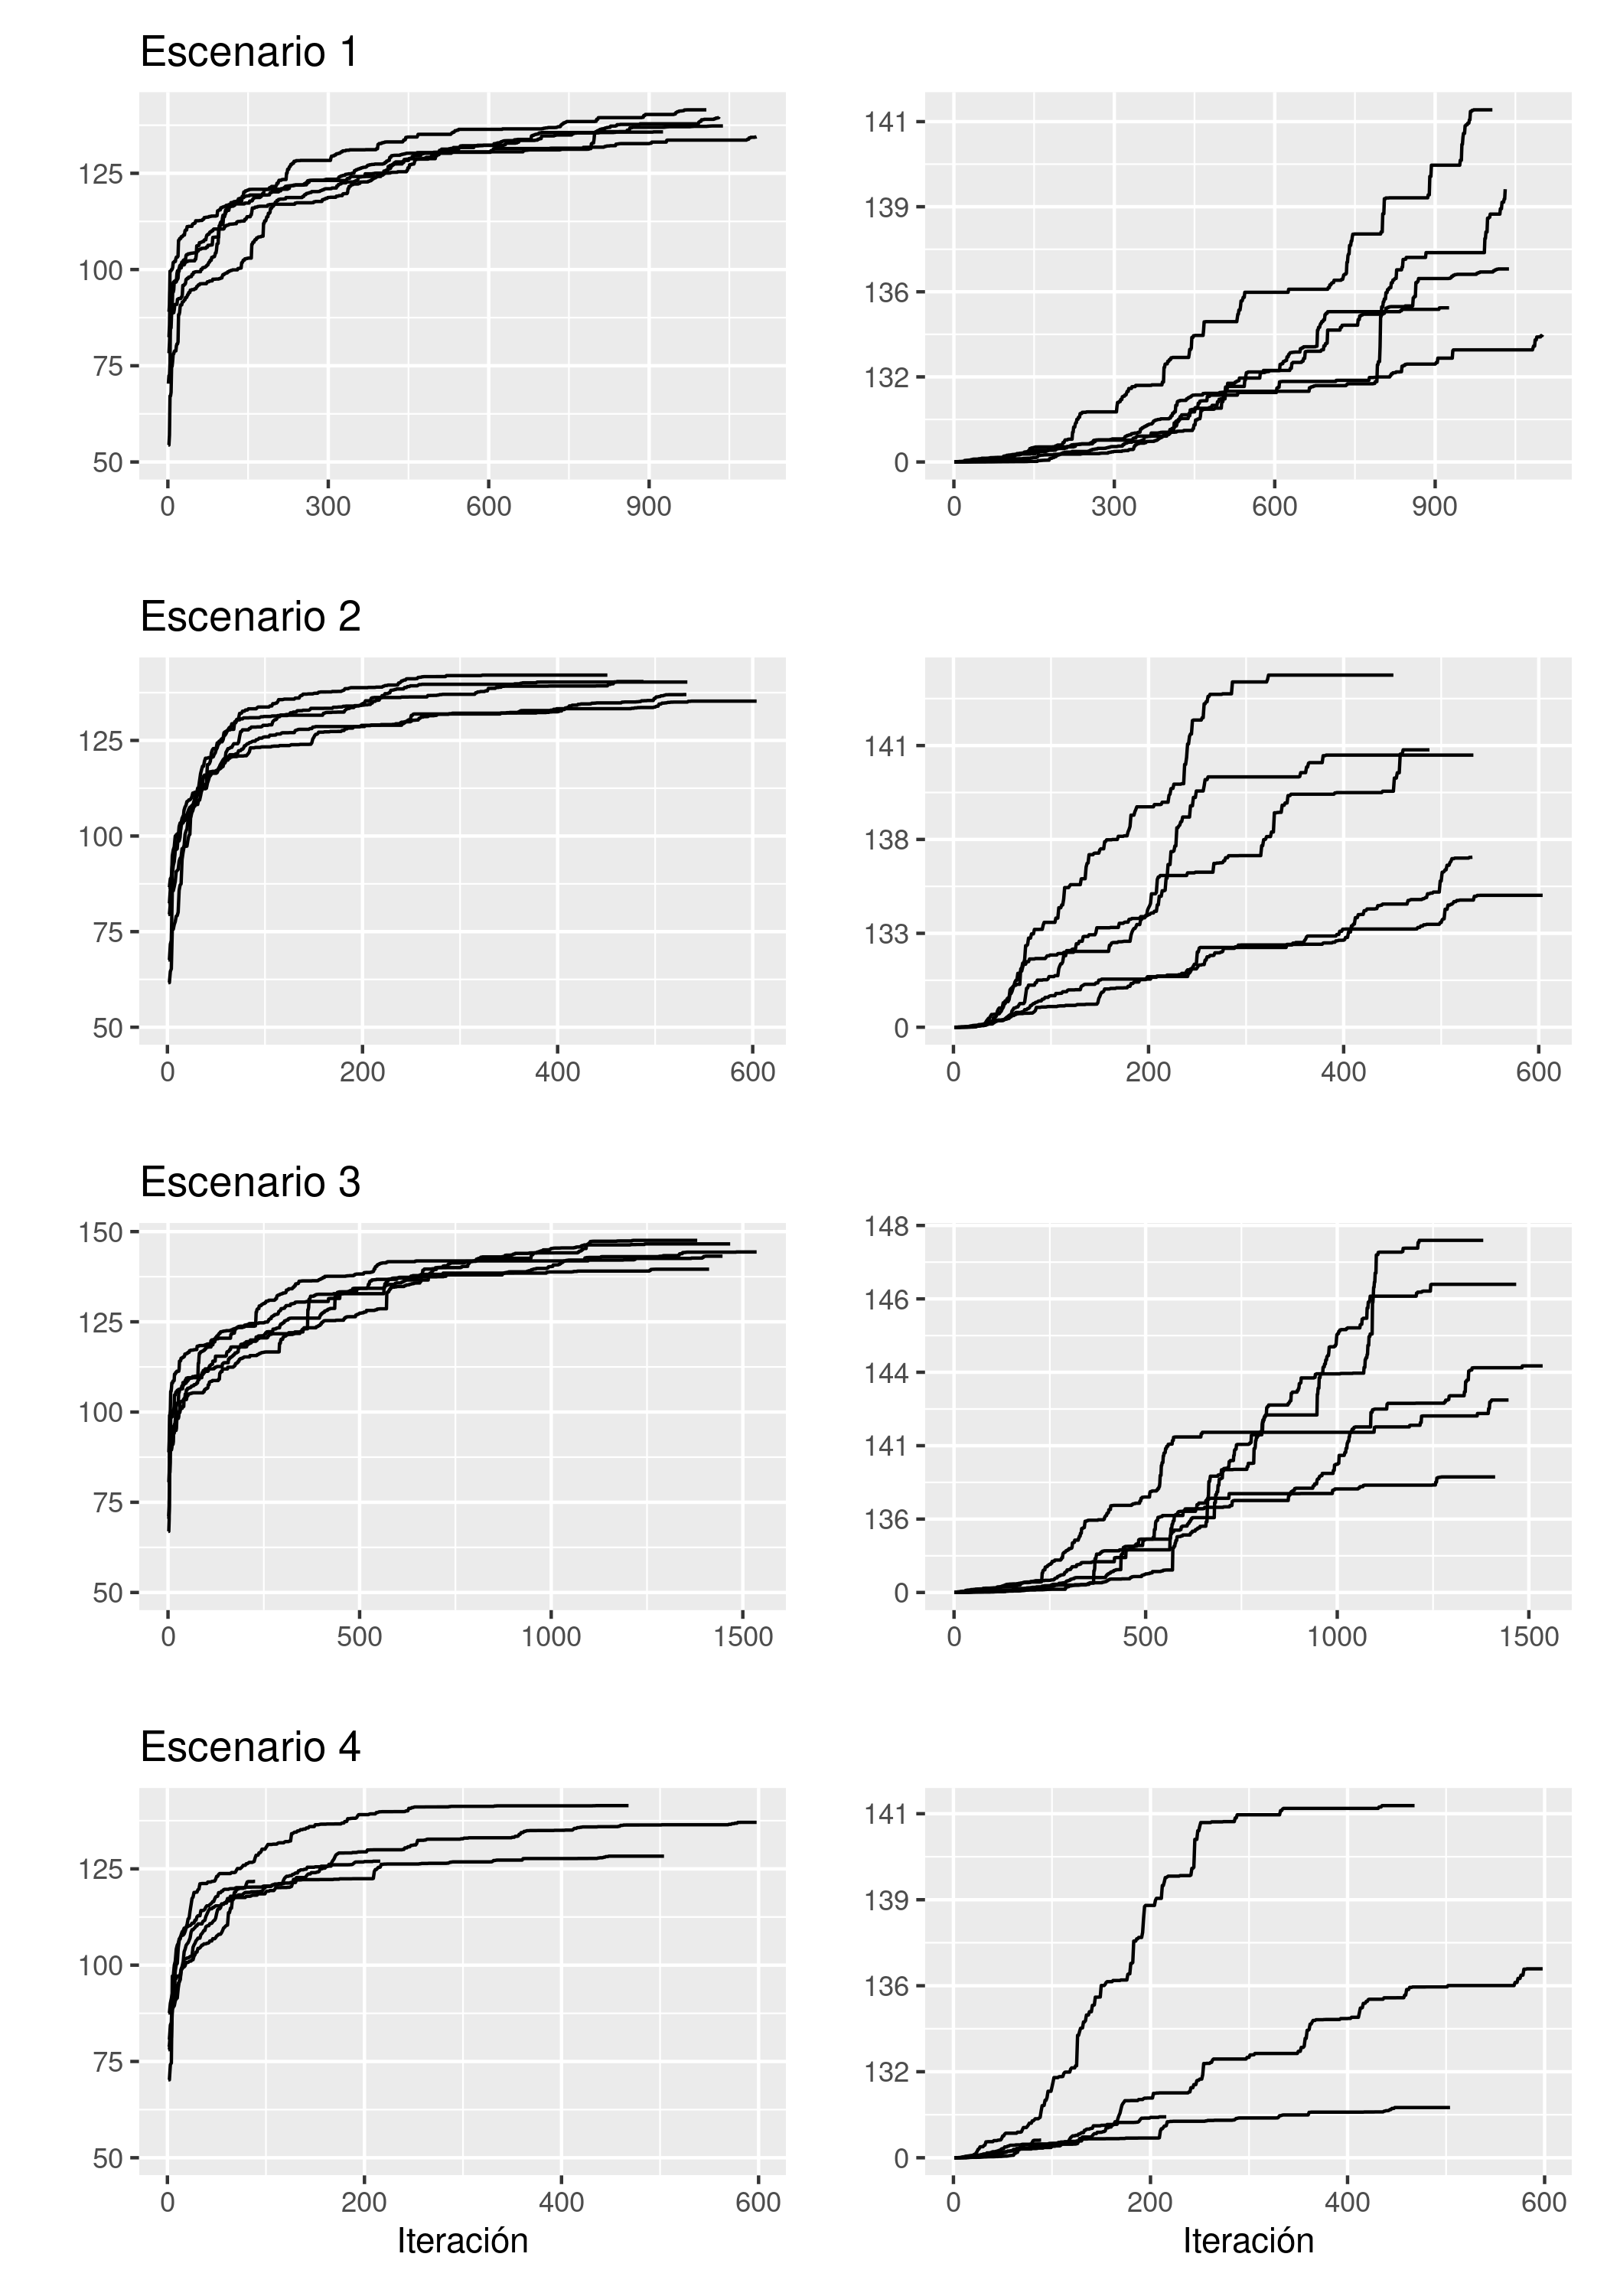
\includegraphics[width=200px]{fig/mixed} \caption{\label{fig:mixed}Evolución de las distintas ejecuciones para la recogida de residuos plásticos. Cada línea representa la función objetivo de la mejor solución para cada iteración de una ejecución. Los gráficos de la columna de la derecha muestran los valor originales de la función objetivo y los de la izquierda, transformado para facilitar la lectura}\label{fig:unnamed-chunk-1}
\end{figure}

\begin{figure}
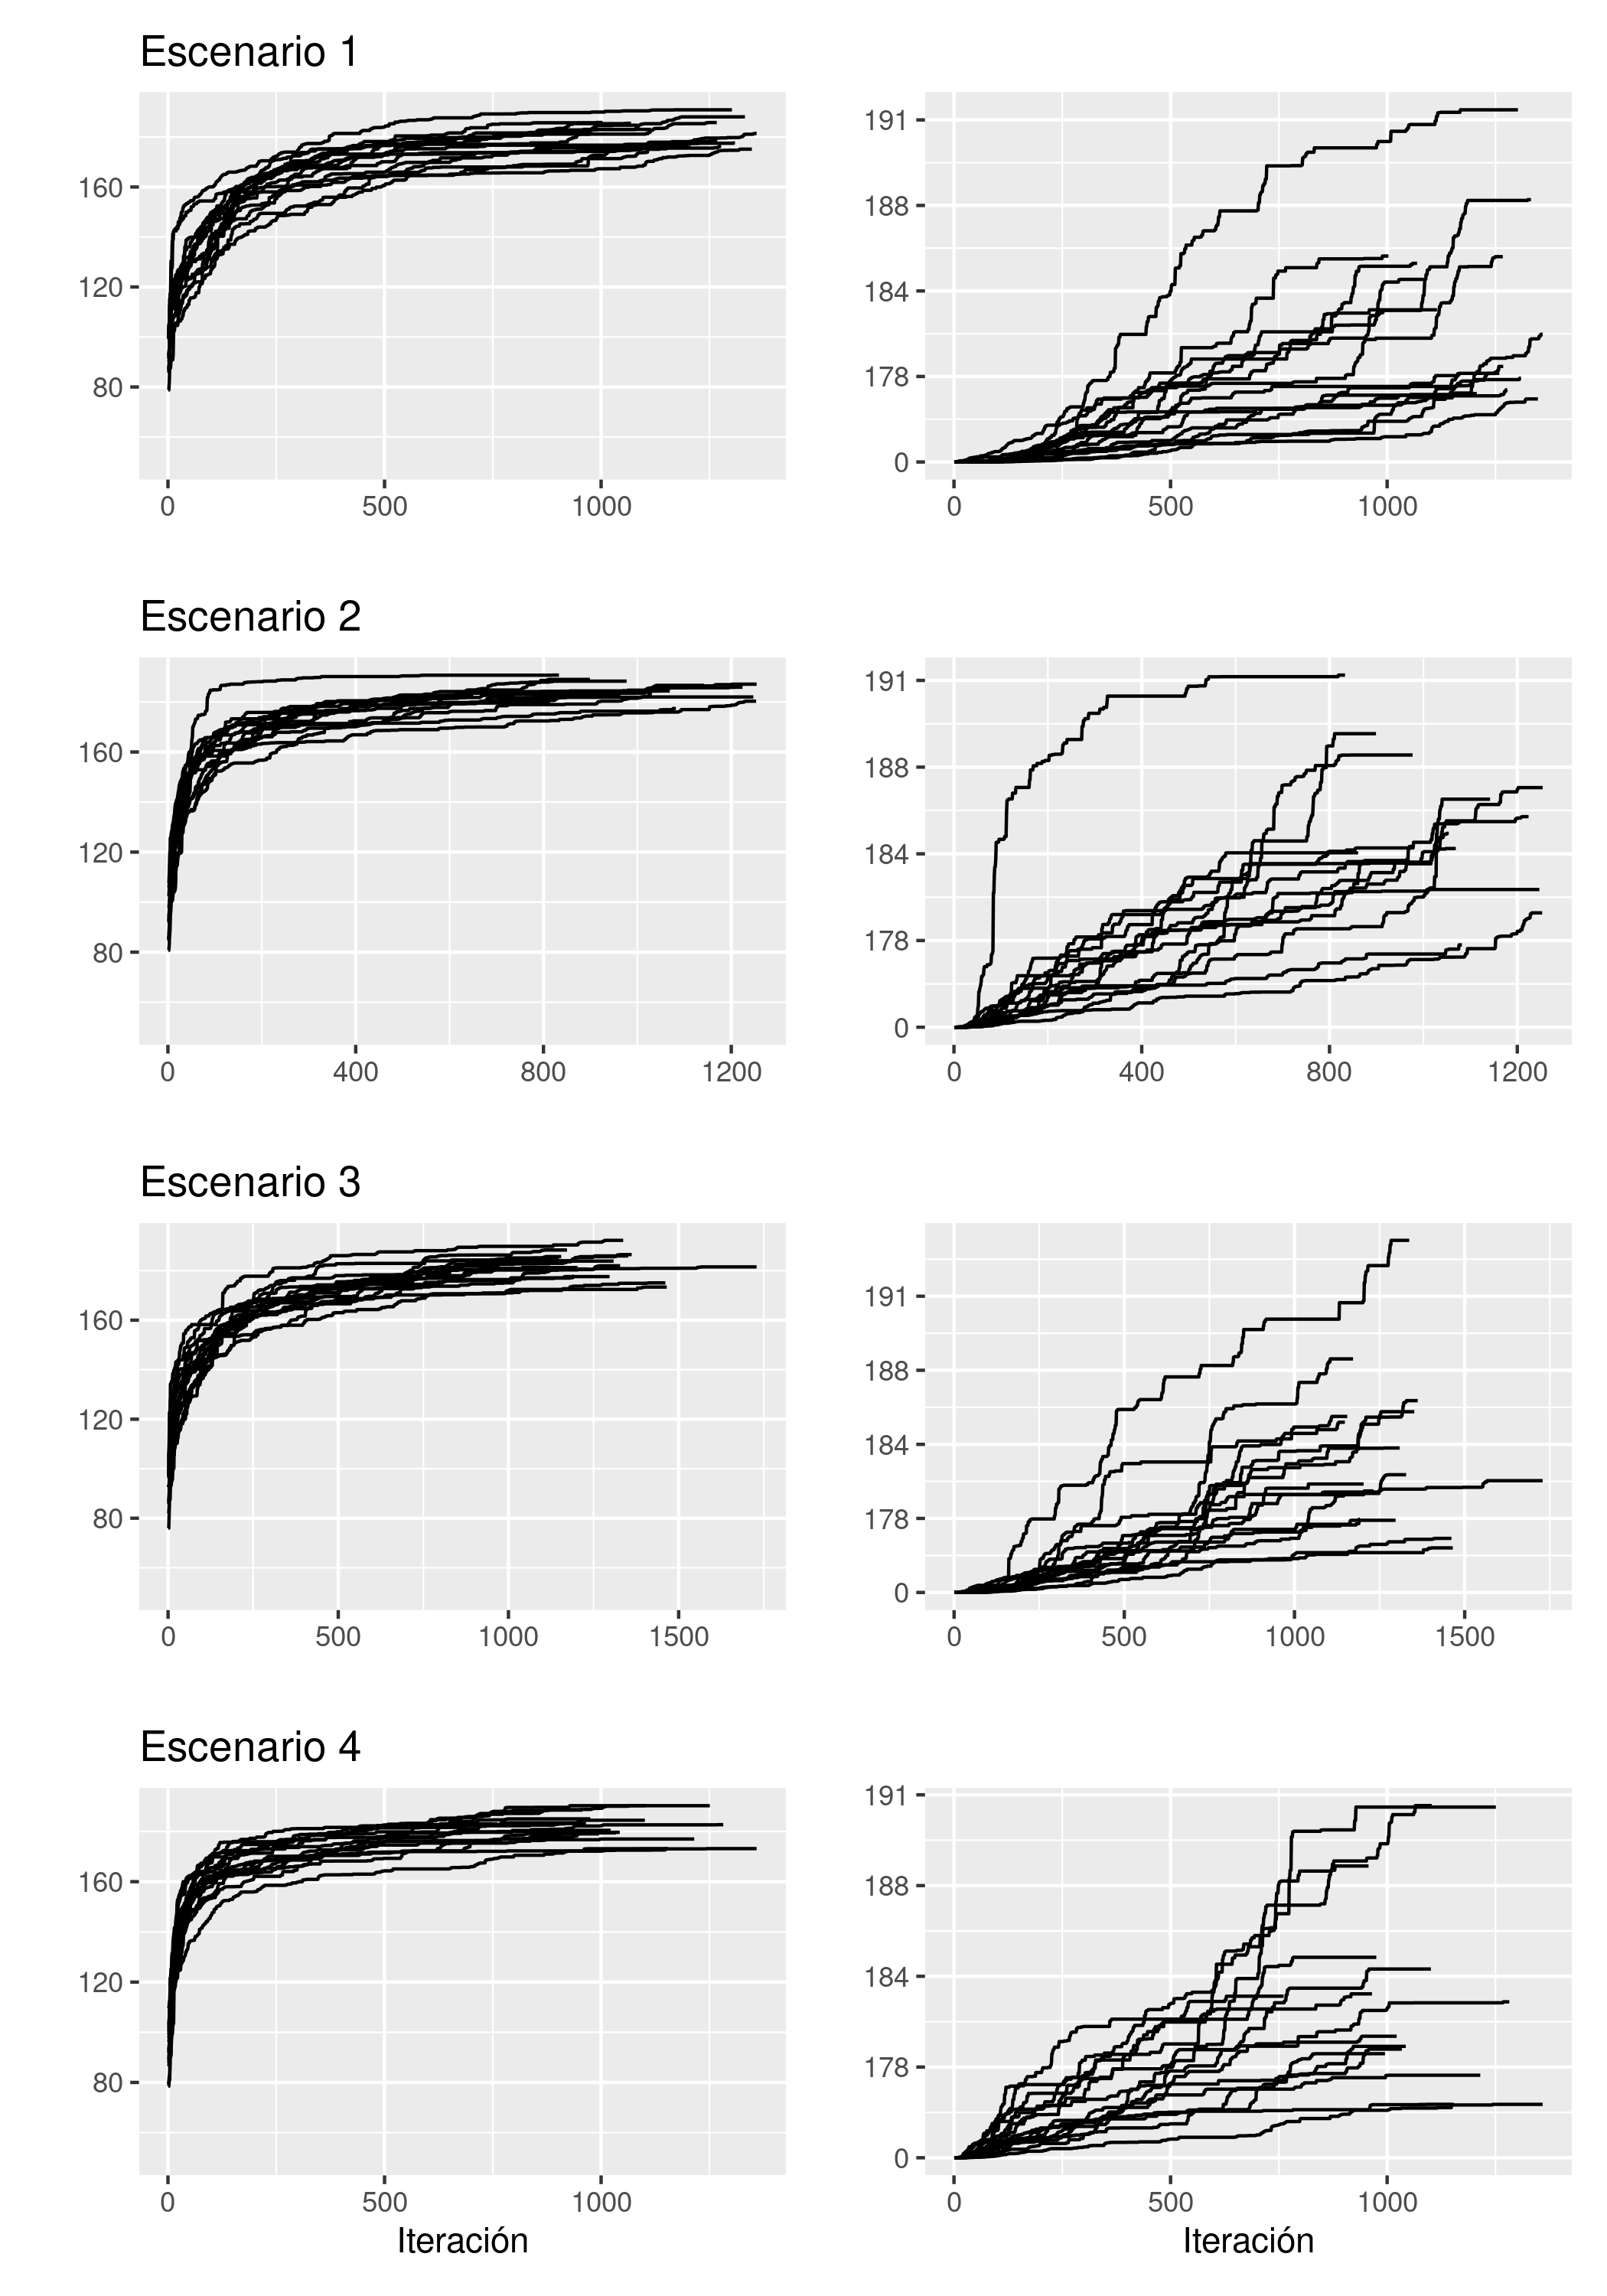
\includegraphics[width=200px]{fig/paper} \caption{\label{fig:paper}Evolución de las distintas ejecuciones para la recogida de residuos de cartón y papel. Cada línea representa la función objetivo de la mejor solución para cada iteración de una ejecución. Los gráficos de la columna de la derecha muestran los valor originales de la función objetivo y los de la izquierda, transformado para facilitar la lectura}\label{fig:unnamed-chunk-2}
\end{figure}

\hypertarget{nivel-de-llenado-aleatorio.}{%
\subsubsection{Nivel de llenado
aleatorio.}\label{nivel-de-llenado-aleatorio.}}

Los indicadores discutidos en la sección anterior no nos permiten
comparar adecuadamente las ejecuciones cuando el nivel de llenado
inicial se obtiene de forma aleatoria. Para la comparativa se ha
calculado el ratio entre la cantidad total de residuo recogido (función
objetivo) y la cantidad de residuo que generaría cada punto de recogida
en el horizonte temporal.

En las tablas X y X se pueden ver los resultados para los residuos
amarillos y azul, respectivamente. Como puede verse, no se parecian
diferencias significativas entre los distintos escenarios.

\textbf{MIXED}

\begin{longtable}[]{@{}ll@{}}
\toprule
& \% recogido\tabularnewline
\midrule
\endhead
Escenario 1 & \(66.43\% \pm 1.54\)\tabularnewline
Escenario 2 & \(68.35\% \pm 2.41\)\tabularnewline
Escenario 3 & \(68.35\% \pm 4.44\)\tabularnewline
Escenario 4 & \(67.69\% \pm 1.9\)\tabularnewline
\bottomrule
\end{longtable}

\textbf{PAPER}

\begin{longtable}[]{@{}ll@{}}
\toprule
& \% recogido\tabularnewline
\midrule
\endhead
Escenario 1 & \(56.03\% \pm 11.9\)\tabularnewline
Escenario 2 & \(59.04\% \pm 2.51\)\tabularnewline
Escenario 3 & \(59.89\% \pm 0.58\)\tabularnewline
Escenario 4 & \(59.89\% \pm 0.58\)\tabularnewline
\bottomrule
\end{longtable}

\hypertarget{conclusiones-y-trabajo-futuro}{%
\section{Conclusiones y trabajo
futuro}\label{conclusiones-y-trabajo-futuro}}

\hypertarget{referencias}{%
\section*{Referencias}\label{referencias}}
\addcontentsline{toc}{section}{Referencias}

\hypertarget{refs}{}
\leavevmode\hypertarget{ref-birattari_classification_2001}{}%
Birattari, Mauro, Luis Paquete, Thomas Stützle, and Klaus Varrentrapp.
2001. ``Classification of Metaheuristics and Design of Experiments for
the Analysis of Components.'' \emph{Teknik Rapor, AIDA-01-05}.

\leavevmode\hypertarget{ref-dantzig_truck_1959}{}%
Dantzig, G. B., and J. H. Ramser. 1959. ``The Truck Dispatching
Problem.'' \emph{Management Science} 6 (1): 80--91.
\url{https://doi.org/10.1287/mnsc.6.1.80}.

\leavevmode\hypertarget{ref-exposito-marquez_greedy_2019}{}%
Expósito-Márquez, Airam, Christopher Expósito-Izquierdo, Julio
Brito-Santana, and J. Andrés Moreno-Pérez. 2019. ``Greedy Randomized
Adaptive Search Procedure to Design Waste Collection Routes in La
Palma.'' \emph{Computers \& Industrial Engineering} 137 (November):
106047. \url{https://doi.org/10.1016/j.cie.2019.106047}.

\leavevmode\hypertarget{ref-flood_traveling-salesman_1956}{}%
Flood, Merrill M. 1956. ``The Traveling-Salesman Problem.''
\emph{Operations Research} 4 (1): 61--75.
\url{https://doi.org/10.1287/opre.4.1.61}.

\leavevmode\hypertarget{ref-gendreau_handbook_2010}{}%
Gendreau, Michel, and Jean-Yves Potvin, eds. 2010. \emph{Handbook of
Metaheuristics}. Vol. 146. International Series in Operations Research
\& Management Science. Boston, MA: Springer US.
\url{https://doi.org/10.1007/978-1-4419-1665-5}.

\leavevmode\hypertarget{ref-glover_tabu_1989}{}%
Glover, Fred. 1989. ``Tabu Search---Part I.'' \emph{ORSA Journal on
Computing} 1 (3): 190--206. \url{https://doi.org/10.1287/ijoc.1.3.190}.

\leavevmode\hypertarget{ref-golden_vehicle_2008}{}%
Golden, Bruce, S. Raghavan, and Edward A. Wasil, eds. 2008. \emph{The
Vehicle Routing Problem: Latest Advances and New Challenges}. Operations
Research/Computer Science Interfaces Series 43. New York, NY: Springer.

\leavevmode\hypertarget{ref-gendreau_variable_2010}{}%
Hansen, Pierre, Nenad Mladenović, Jack Brimberg, and José A. Moreno
Pérez. 2010. ``Variable Neighborhood Search.'' In \emph{Handbook of
Metaheuristics}, edited by Michel Gendreau and Jean-Yves Potvin,
146:61--86. Boston, MA: Springer US.
\url{https://doi.org/10.1007/978-1-4419-1665-5_3}.

\leavevmode\hypertarget{ref-helsgaun_effective_2000}{}%
Helsgaun, Keld. 2000. ``An Effective Implementation of the
Lin--Kernighan Traveling Salesman Heuristic.'' \emph{European Journal of
Operational Research} 126 (1): 106--30.
\url{https://doi.org/10.1016/S0377-2217(99)00284-2}.

\leavevmode\hypertarget{ref-lin_survey_2014}{}%
Lin, Canhong, K. L. Choy, G. T. S. Ho, S. H. Chung, and H. Y. Lam. 2014.
``Survey of Green Vehicle Routing Problem: Past and Future Trends.''
\emph{Expert Systems with Applications} 41 (4): 1118--38.
\url{https://doi.org/10.1016/j.eswa.2013.07.107}.

\leavevmode\hypertarget{ref-mladenovic_variable_1997}{}%
Mladenović, N., and P. Hansen. 1997. ``Variable Neighborhood Search.''
\emph{Computers \& Operations Research} 24 (11): 1097--1100.
\url{https://doi.org/10.1016/S0305-0548(97)00031-2}.

\leavevmode\hypertarget{ref-du_traveling_2007}{}%
Punnen, Abraham P. 2007. ``The Traveling Salesman Problem: Applications,
Formulations and Variations.'' In \emph{The Traveling Salesman Problem
and Its Variations}, edited by Gregory Gutin and Abraham P. Punnen,
12:1--28. Boston, MA: Springer US.
\url{https://doi.org/10.1007/0-306-48213-4_1}.

\leavevmode\hypertarget{ref-sorensen_metaheuristics-metaphor_2015}{}%
Sörensen, Kenneth. 2015. ``Metaheuristics-the Metaphor Exposed.''
\emph{International Transactions in Operational Research} 22 (1): 3--18.
\url{https://doi.org/10.1111/itor.12001}.

\end{document}
